

\documentclass[letterpaper,12pt]{article} %Modifica el tipo de documento y el tamaño de la letra.
\usepackage[utf8]{inputenc} %Formato UTF-8 para caracteres especiales.
\usepackage[shortlabels]{enumitem}
\usepackage[spanish,mexico]{babel} 
\usepackage{amsmath,amssymb,amsfonts,latexsym,cancel}
\usepackage{hyperref}
\usepackage{wrapfig}
\usepackage[rflt]{floatflt}
\usepackage[pdftex]{graphicx}
\usepackage{fancyhdr} %Paquete para el header y el formato de la portada. 
\usepackage{float}
\usepackage{longtable,multirow,booktabs}
\usepackage{cite}
\usepackage{wrapfig}
\usepackage[square,numbers]{natbib}
\usepackage{multicol}
\usepackage{caption}
\usepackage[]{sidecap}
\usepackage{adjustbox}
\usepackage{parskip}
\usepackage{enumitem}
\usepackage{tikz}
\usepackage{lipsum}
\usepackage[]{xcolor}



%Fin de Préambulo


%Inicio formato de Página. 

\textheight = 21cm %Medidas de la  página
\textwidth = 18cm  %Medidas de la página
\topmargin = -2cm  %Medidas de la página    
\oddsidemargin = -0.8cm %Medidas de la página
\pagestyle{fancy} %Diseño de la página


\fancyhf{}
\lhead{Facultad de Ciencias}%%LeftHead
\chead{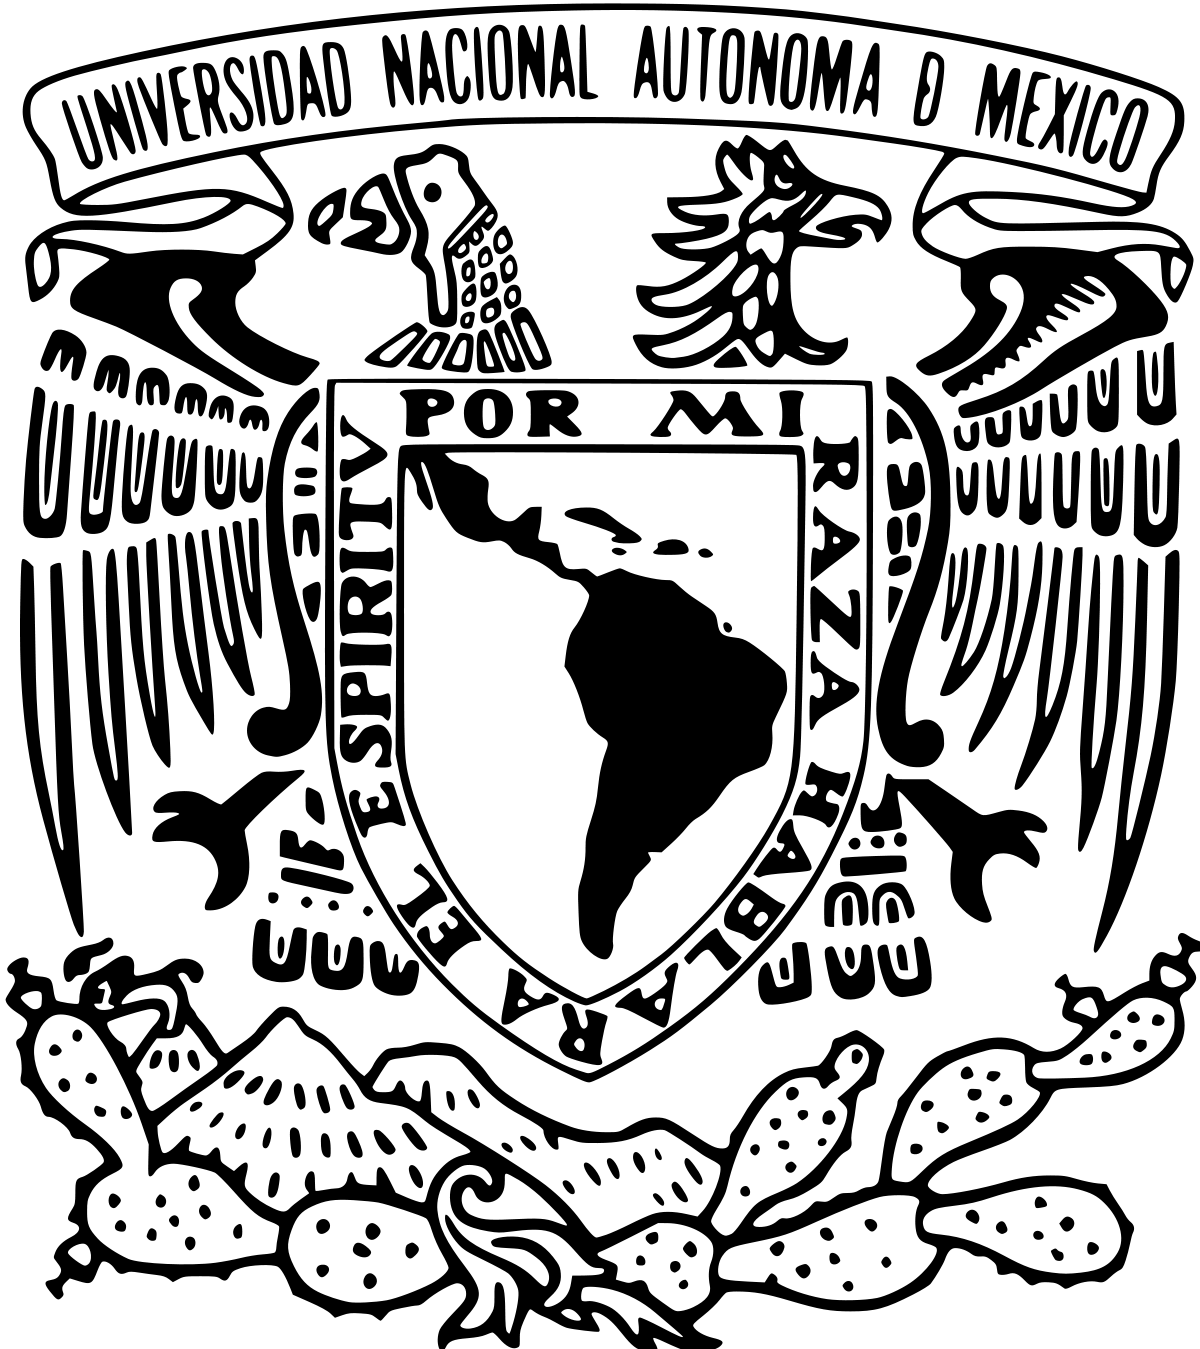
\includegraphics[width=1cm, height=1cm]{Imágenes/UNAM.png}}%%CenterHead
%\lfoot{USM}
\rhead{Heurísticas de Optimización Combinatoria}%%RightHead

\setlength{\columnsep}{4mm}%Comandos para el formato de la página.
%\setlength{\parindent}{4em}%Sangría al comenzar un nuevo párrafo.
\setlength{\parindent}{0.5in}
%\setlength{\parindent}{4em}%Sangría al comenzar un nuevo párrafo.
\setlength{\parskip}{1em}%Distancia entre párrafos.
\renewcommand{\baselinestretch}{1.5}% Espacio entre línea y línea o interlineado.
\setlength{\headheight}{33pt}

%Fin formato de Página

%Aquí inicia el documento. 
\begin{document}
    \thispagestyle{empty}
			\begin{figure}[ht]
		   \minipage{0.87\textwidth}
				
\includegraphics[width=3cm]{Imágenes/ciencias.jpg}
				\label{escudoFI}
		   \endminipage
		   \minipage{0.32\textwidth}
				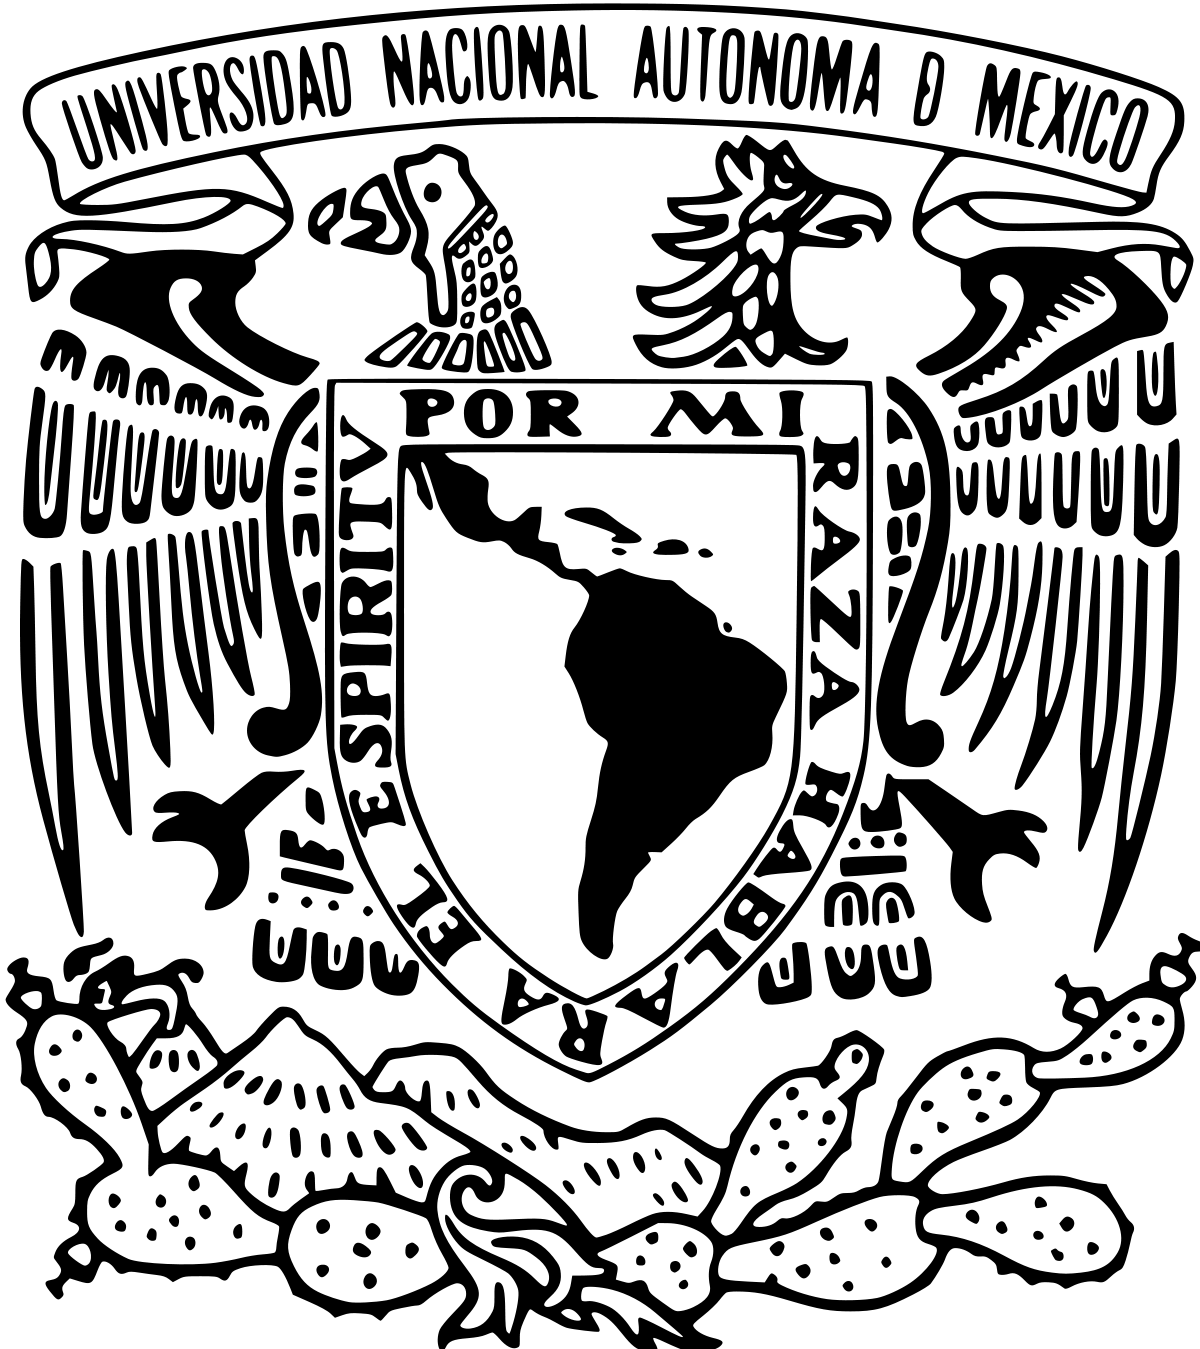
\includegraphics[height = 2.25cm ,width=2cm]{Imágenes/UNAM.png}
				\label{EscuoUNAM}
			\endminipage
				%%\vspace{-1cm}
		\end{figure}
		
		\vspace{0.1cm}
		
		\begin{center}
		    {\scshape\LARGE \textbf{Universidad Nacional Autónoma de México} \par}
			{\scshape\Large Facultad de Ciencias\par}
            
             {\LARGE Heurísticas de Optimización Combinatoria}

			% Restauramos el interlineado:
			\begin{center}
			
			{\LARGE \textit{Grupo: 7167 - Semestre: 2027-1}}

            
                {\LARGE  \bfseries{Lectura 01} \\}
			{\LARGE\bfseries Problema del Agente Viajero mediante Aceptación por Umbrales\par}

		{\scshape\Large Fecha de entrega: 18/09/2026\par}	

			        \LARGE	{ \textbf{Profesor:}}\\
        \large		{Canek Peláez Valdés}
       
		\vspace{-0.5cm}	
		
		\LARGE	{ \textbf{Alumna:}}\\

        \normalsize	 {Carpinteiro Tapia Mariam Ximena}
        
        \vspace{-0.5cm}
        
       
        
        

				\vspace{1.25cm}
				\vspace{0.9cm}
				
			\end{center}
	
		\end{center}
    \newpage


\section{Abstract}

Presentamos la implementación de la heurística de Aceptación por Umbrales
(\textit{Threshold Accepting}) para resolver instancias del Problema del Agente
Viajero (TSP). Dada una gráfica no completa de ciudades con distancias
geográficas, se busca la trayectoria de menor costo que visite un subconjunto
de ellas, penalizando las aristas inexistentes para favorecer soluciones
factibles. El sistema se implementó en C++ con una función de costo evaluable
en tiempo constante por vecino mediante evaluación incremental, y se
paralelizó la experimentación sobre miles de semillas. Para las instancias de
prueba de 40 y 150 ciudades se obtuvieron soluciones factibles con costos
normalizados de $0.2659$ y $0.1400$ respectivamente.

\section{Introducción}

El Problema del Agente Viajero (TSP, por sus siglas en inglés) es uno de los
problemas clásicos de optimización combinatoria y pertenece a la clase de
problemas NP-duros: no se conoce un algoritmo que encuentre la solución óptima
en tiempo polinomial. Por ello, para instancias de tamaño no trivial se recurre
a heurísticas, las cuales dejan un poco de lado la optimalidad a cambio de encontrar
soluciones suficientemente buenas en un tiempo razonable.

En este trabajo se aborda una variante del TSP: dado un subconjunto de ciudades
sobre un mapa, se busca la trayectoria más corta que pase por todas ellas. La
gráfica de ciudades es densa pero no completa, de modo que no toda trayectoria
es válida; una parte central del problema es precisamente distinguir y favorecer
las soluciones factibles.

Se implementa la heurística de Aceptación por Umbrales, una variante del
Recocido Simulado propuesta por Dueck y Scheuer en 1990, y realizamos
experimentación computacional para calibrar sus parámetros y evaluar la calidad
de las soluciones obtenidas sobre dos instancias de prueba, de 40 y 150
ciudades.

\section{El problema}

Empecemos decribiendo el problema, la instancia se modela mediante una gráfica ponderada $G(V, E)$, donde los
vértices son ciudades y las aristas representan conexiones entre ellas, con un
peso igual a la distancia geográfica. Esta gráfica es densa pero {no
completa}, es decir que existen pares de ciudades sin conexión directa.

Sea $S \subseteq V$ el subconjunto de ciudades a visitar. Para simplificar la
optimización se trabaja sobre la gráfica completa $G_S$ inducida por $S$, con
una función de peso aumentada $w_S$: si la arista existe en $E$ se usa su
distancia real; si no, se asigna un peso deliberadamente grande, igual a la
distancia natural multiplicada por la distancia máxima de $S$. Este castigo hace que las soluciones con aristas inexistentes tengan un costo muy alto, de modo que la heurística tiende a descartarlas.

Cualquier permutación de $S$ es una solución en $G_S$, pero se distinguen dos
tipos: \textbf{factibles}, aquellas cuyas aristas consecutivas existen todas en
$E$; y \textbf{no factibles}, las que usan al menos una arista inexistente.

\subsection{Distancia natural}

Para las aristas que no aparecen en la base de datos, la distancia se calcula
con la fórmula del gran círculo (\textit{haversine}), suponiendo la Tierra una
esfera de radio $R = 6{,}373{,}000$ metros. Dadas dos ciudades $u$ y $v$ con
coordenadas en latitud y longitud:
\[
    d(u,v) = R \cdot 2 \arctan\!\left(\frac{\sqrt{A}}{\sqrt{1-A}}\right),
\]
donde $A$ combina las diferencias de latitud y longitud convertidas a radianes.

\subsection{Función de costo}

El costo de una trayectoria $P = v_{\rho(1)}, \dots, v_{\rho(k)}$ es la suma de
los pesos aumentados de sus aristas consecutivas, normalizada:
\[
    f(P) = \frac{\sum_{i=2}^{k} w_S(v_{\rho(i-1)}, v_{\rho(i)})}{N(S)}.
\]
El normalizador $N(S)$ es la suma de las $k-1$ aristas reales más pesadas entre
ciudades de $S$. Con esta normalización, toda solución factible se evalúa en el
intervalo $[0, 1]$, mientras que las no factibles superan $1$.

\section{La heurística: Aceptación por Umbrales}

La Aceptación por Umbrales (\textit{Threshold Accepting}), propuesta por Dueck y
Scheuer en 1990, es una variante simplificada del Recocido Simulado. Parte de
una solución inicial y una temperatura $T$, y de forma iterativa propone una
solución vecina $s'$, aceptándola cuando
\[
    f(s') \leq f(s) + T.
\]
Es decir, acepta toda mejora y también empeoramientos pequeños, acotados por el
umbral $T$. Esta tolerancia controlada a empeorar es lo que nos permite escapar de
mínimos locales.

La temperatura desciende de forma gradual, el descenso se organiza en
\textbf{lotes}: un lote es un número fijo $L$ de soluciones aceptadas. Se
ejecutan lotes a una misma temperatura mientras el promedio de sus costos siga
mejorando (equilibrio térmico); cuando deja de mejorar, la temperatura se enfría
multiplicándola por un factor $\varphi \in (0,1)$. El proceso termina cuando
$T$ cae por debajo de un cero virtual $\varepsilon$. A lo largo de toda la
ejecución se conserva la mejor solución encontrada.

\subsection{Vecindad}

Dos soluciones son vecinas si una se obtiene de la otra intercambiando dos
elementos de la permutación. Para una instancia de $k$ ciudades existen
$\binom{k}{2} = k(k-1)/2$ vecinos posibles de cada solución.

\subsection{Temperatura inicial}

La temperatura inicial se calcula mediante búsqueda binaria: se busca un valor de
$T$ para el cual se acepte un porcentaje $P$ elevado de vecinos de un escenario
inicial (se usó $P = 0.9$). Primero se acota un intervalo duplicando o
reduciendo $T$ a la mitad hasta rodear el objetivo, y luego se aplica búsqueda binaria sobre ese intervalo hasta acercarse a 
P.

\section{Diseño de la solución}

El sistema se estructuró en componentes con responsabilidades separadas:

\begin{itemize}
    \item \textbf{Lectura y datos.} Un lector interpreta los archivos de
    instancia \texttt{.tsp}, y una capa de acceso a la base de datos SQLite
    recupera las ciudades y las conexiones. La gráfica real solo se consulta una
    vez, al inicio.

    \item \textbf{Instancia.} La clase \texttt{Instance} reindexa las ciudades
    (cuyos identificadores son dispersos) a índices contiguos $0, \dots, k-1$, y
    construye una matriz de adyacencia $k \times k$ con los pesos aumentados ya
    calculados. La distancia máxima y el normalizador se calculan una única vez
    en el constructor, pues no dependen del orden de la trayectoria.

    \item \textbf{Solución.} La clase \texttt{Solution} representa una
    permutación con su costo, y sabe generar un vecino (intercambio de dos
    posiciones) y deshacerlo.

    \item \textbf{Heurística.} La clase \texttt{ThresholdAccepting} orquesta la
    búsqueda: lotes, enfriamiento y conservación de la mejor solución. No conoce
    los detalles de la gráfica ni de la base de datos.
\end{itemize}

Esta separación permite probar cada pieza de forma aislada mediante pruebas
unitarias, y sustituir la heurística sin tocar el modelo del problema.

\section{Detalles de implementación}

El sistema se implementó en C++ (estándar C++17), usando SQLite para la base de
datos de ciudades. Se destacan las siguientes decisiones:

\begin{itemize}
    \item \textbf{Matriz de pesos con arreglos.} Los pesos aumentados $w_S$ se
    precalculan en una matriz plana $k \times k$, de modo que evaluar una
    solución es solo acceso a arreglo, sin consultas a la base de datos ni
    cálculos trigonométricos en el ciclo caliente.

    \item \textbf{Evaluación incremental.} Un intercambio de dos posiciones
    altera a lo más cuatro aristas de la trayectoria. En lugar de recalcular la
    suma completa ($O(k)$), se restan las aristas viejas y se suman las nuevas
    ($O(1)$). Para acotar el error de punto flotante acumulado tras millones de
    intercambios, cada cierto número de operaciones se recalcula el costo
    completo.

    \item \textbf{Reproducibilidad.} Toda la aleatoriedad proviene de un
    generador Mersenne Twister con semilla explícita. Una corrida queda
    determinada por completo por su semilla y sus parámetros, lo que permite
    reproducir cualquier resultado y comparar configuraciones de forma justa.

    \item \textbf{Cláusula de escape.} Se implementó un mecanismo opcional de
    recalentamiento: si la mejor solución no mejora durante un número de lotes,
    la temperatura se reinicia para permitir escapar de un mínimo local. Este
    mecanismo aumentó notablemente la proporción de corridas que terminan en
    solución factible, pero no me proporcionaron el mejor costo.

    \item \textbf{Experimentación paralela.} Como cada semilla es independiente,
    los barridos de miles de semillas se ejecutan en paralelo, una por núcleo,
    reduciendo el tiempo total en proporción al número de núcleos disponibles. Además compilamos con optimización (\texttt{-O2}) lo cual redujo el tiempo por corrida.
\end{itemize}

\section{Resultados}

Se resolvieron las dos instancias de prueba, de 40 y 150 ciudades. Los mejores resultados se obtuvieron con los parámetros
$L = 4000$, $\varphi = 0.995$, $\varepsilon = 10^{-5}$ y $P = 0.9$.

\begin{table}[H]
    \centering
    \begin{tabular}{lccc}
        \toprule
        Instancia & Semilla & Costo & Factible \\
        \midrule
        \texttt{input-40}  & 207 & $0.265907$ & Sí \\
        \texttt{input-150} & 337 & $0.140028$ & Sí \\
        \bottomrule
    \end{tabular}
    \caption{Mejores soluciones encontradas para cada instancia.}
\end{table}

Ambas soluciones son factibles, es decir, su costo normalizado es menor que $1$
y todas sus aristas existen en la gráfica real. Como referencia, la trayectoria
trivial (las ciudades en orden de identificador) no es factible en ninguna de
las dos instancias, con evaluaciones del orden de millones.

\subsection{Verificación de las soluciones}

Las mejores soluciones se guardaron en archivos \texttt{.tsp} y se
reevaluaron con el programa para confirmar su costo y factibilidad. Las
figuras \ref{fig:build-40} y \ref{fig:build-150} muestran la salida del
programa al reevaluar cada solución: el costo coincide con el reportado durante
la búsqueda y ambas resultan factibles.

\begin{figure}[H]
    \centering
    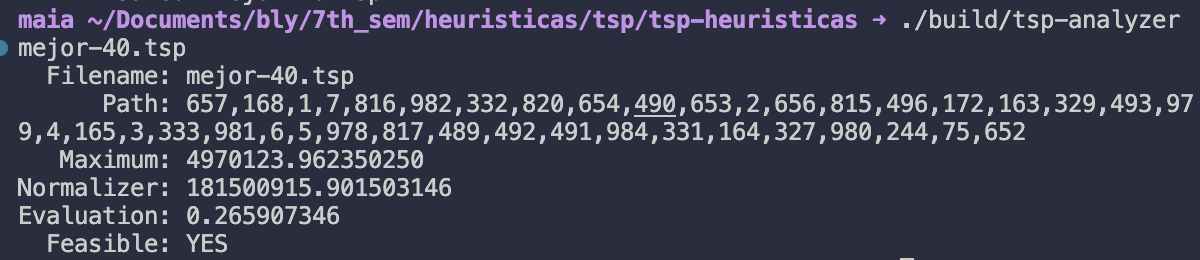
\includegraphics[width=.7\linewidth]{Imágenes/build-40.png}
    \caption{Reevaluación de la mejor solución de \texttt{input-40} (costo $0.265907$).}
    \label{fig:build-40}
\end{figure}

\begin{figure}[H]
    \centering
    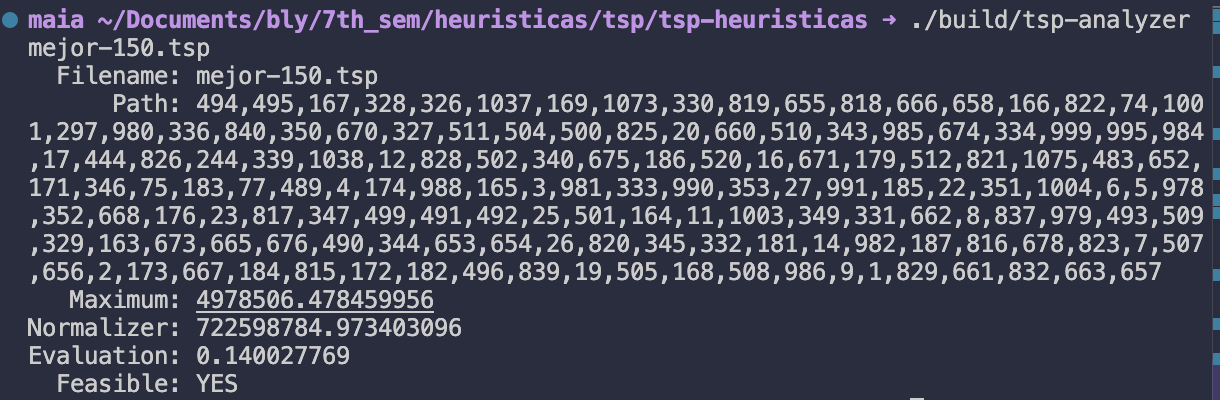
\includegraphics[width=.7\linewidth]{Imágenes/build-150.png}
    \caption{Reevaluación de la mejor solución de \texttt{input-150} (costo $0.140028$).}
    \label{fig:build-150}
\end{figure}

\subsection{Evolución del costo}

Las figuras \ref{fig:trace-40} y \ref{fig:trace-150} muestran la evolución del
costo de la solución aceptada a lo largo de las evaluaciones aceptadas. En ambas
se aprecia el mismo comportamiento: un descenso pronunciado al inicio, cuando la
temperatura es alta y la búsqueda explora aceptando incluso soluciones no
factibles con penalizaciones grandes, seguido de un largo tramo en el que el
costo se estabiliza cerca de su valor final conforme la temperatura disminuye.
La caja en cada gráfica indica el costo de la última solución aceptada, que
puede diferir ligeramente del mejor costo global, pues la heurística conserva
por separado la mejor solución vista durante toda la corrida.

\begin{figure}[H]
    \centering
    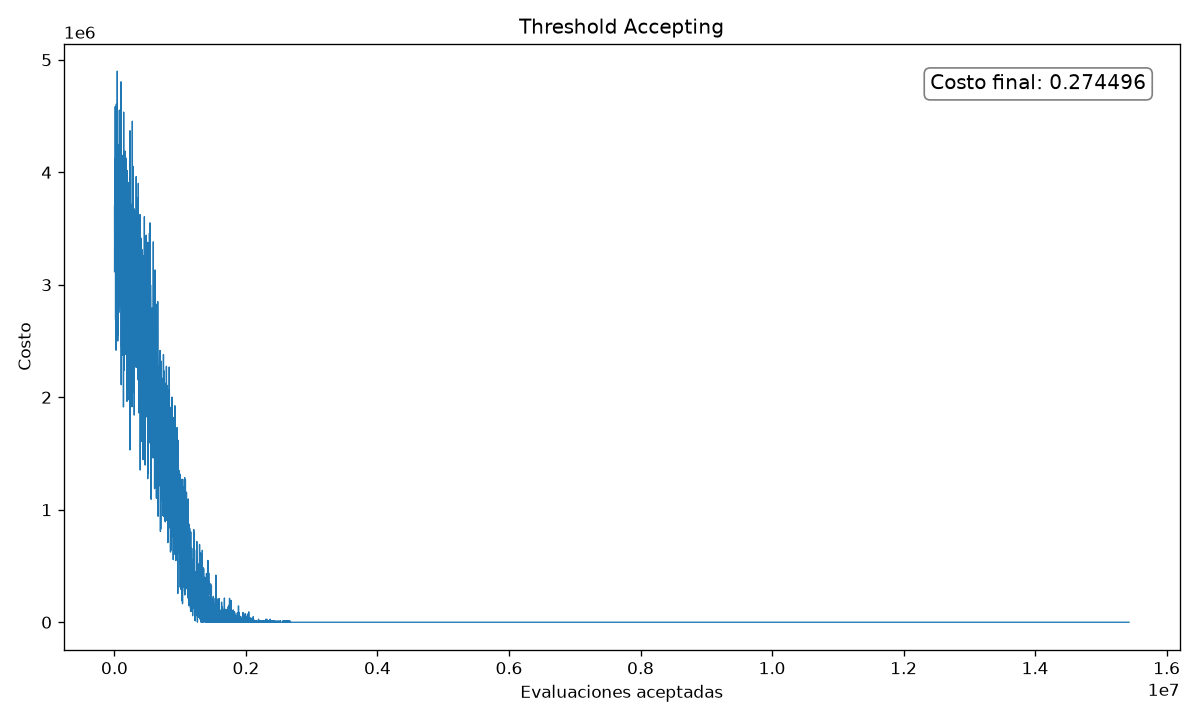
\includegraphics[width=.8\linewidth]{Imágenes/trace-40.png}
    \caption{Evolución del costo para \texttt{input-40} (semilla 207).}
    \label{fig:trace-40}
\end{figure}

\begin{figure}[H]
    \centering
    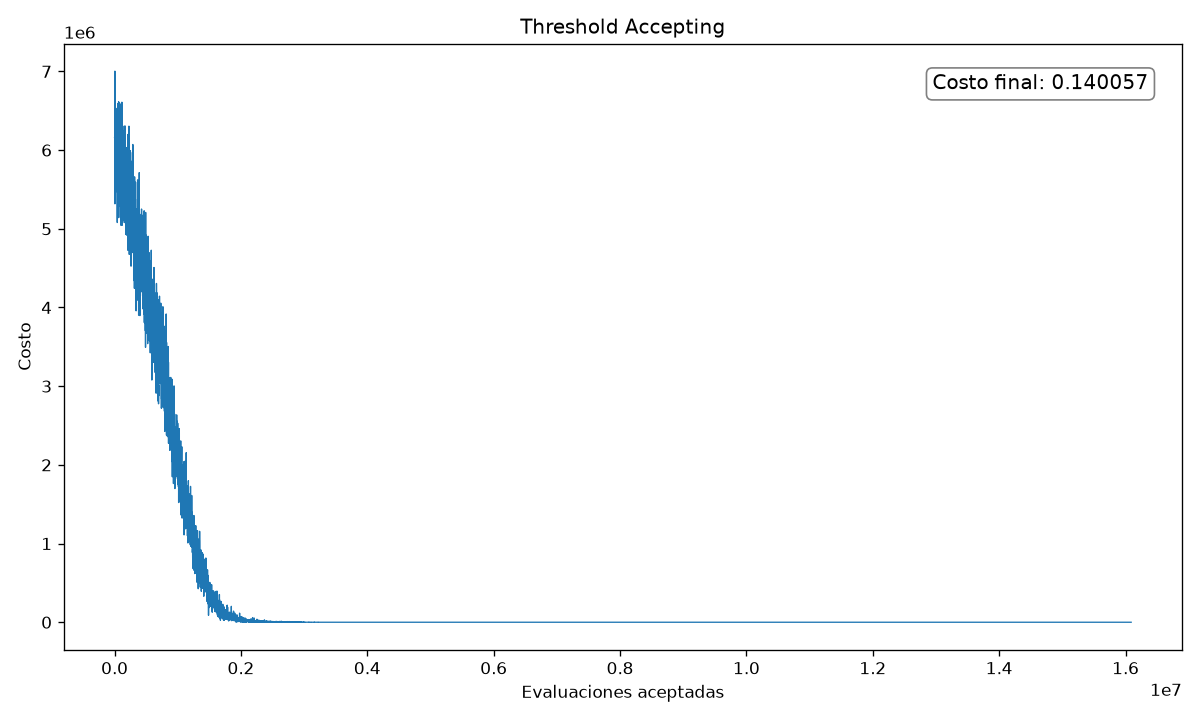
\includegraphics[width=.8\linewidth]{Imágenes/trace-150.png}
    \caption{Evolución del costo para \texttt{input-150} (semilla 337).}
    \label{fig:trace-150}
\end{figure}

\subsection{Trayectorias en el mapa}

Las figuras \ref{fig:mapa-40} y \ref{fig:mapa-150} muestran las mejores
trayectorias trazadas sobre el mapa, ubicando cada ciudad por sus coordenadas.

\begin{figure}[H]
    \centering
    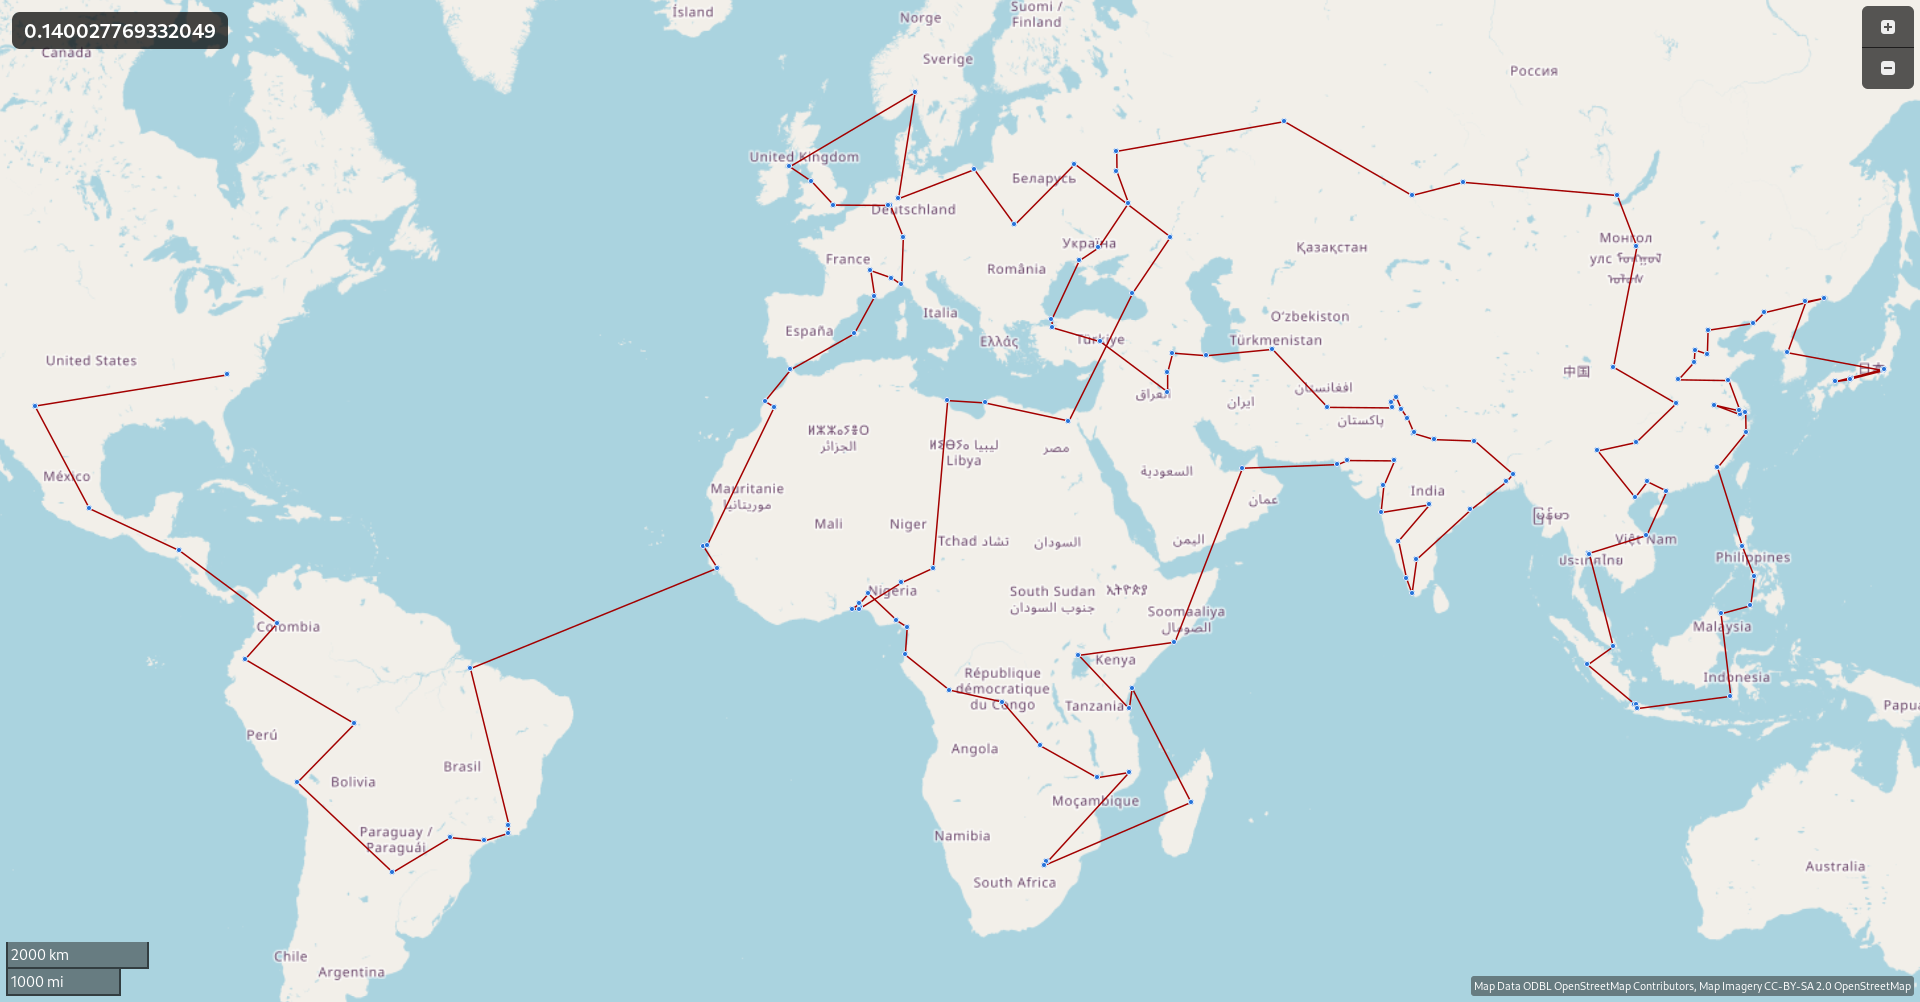
\includegraphics[width=.81\linewidth]{Imágenes/mapa-150.png}
    \caption{Mejor trayectoria para \texttt{input-150}.}
    \label{fig:mapa-150}
\end{figure}

\begin{figure}[H]
    \centering
    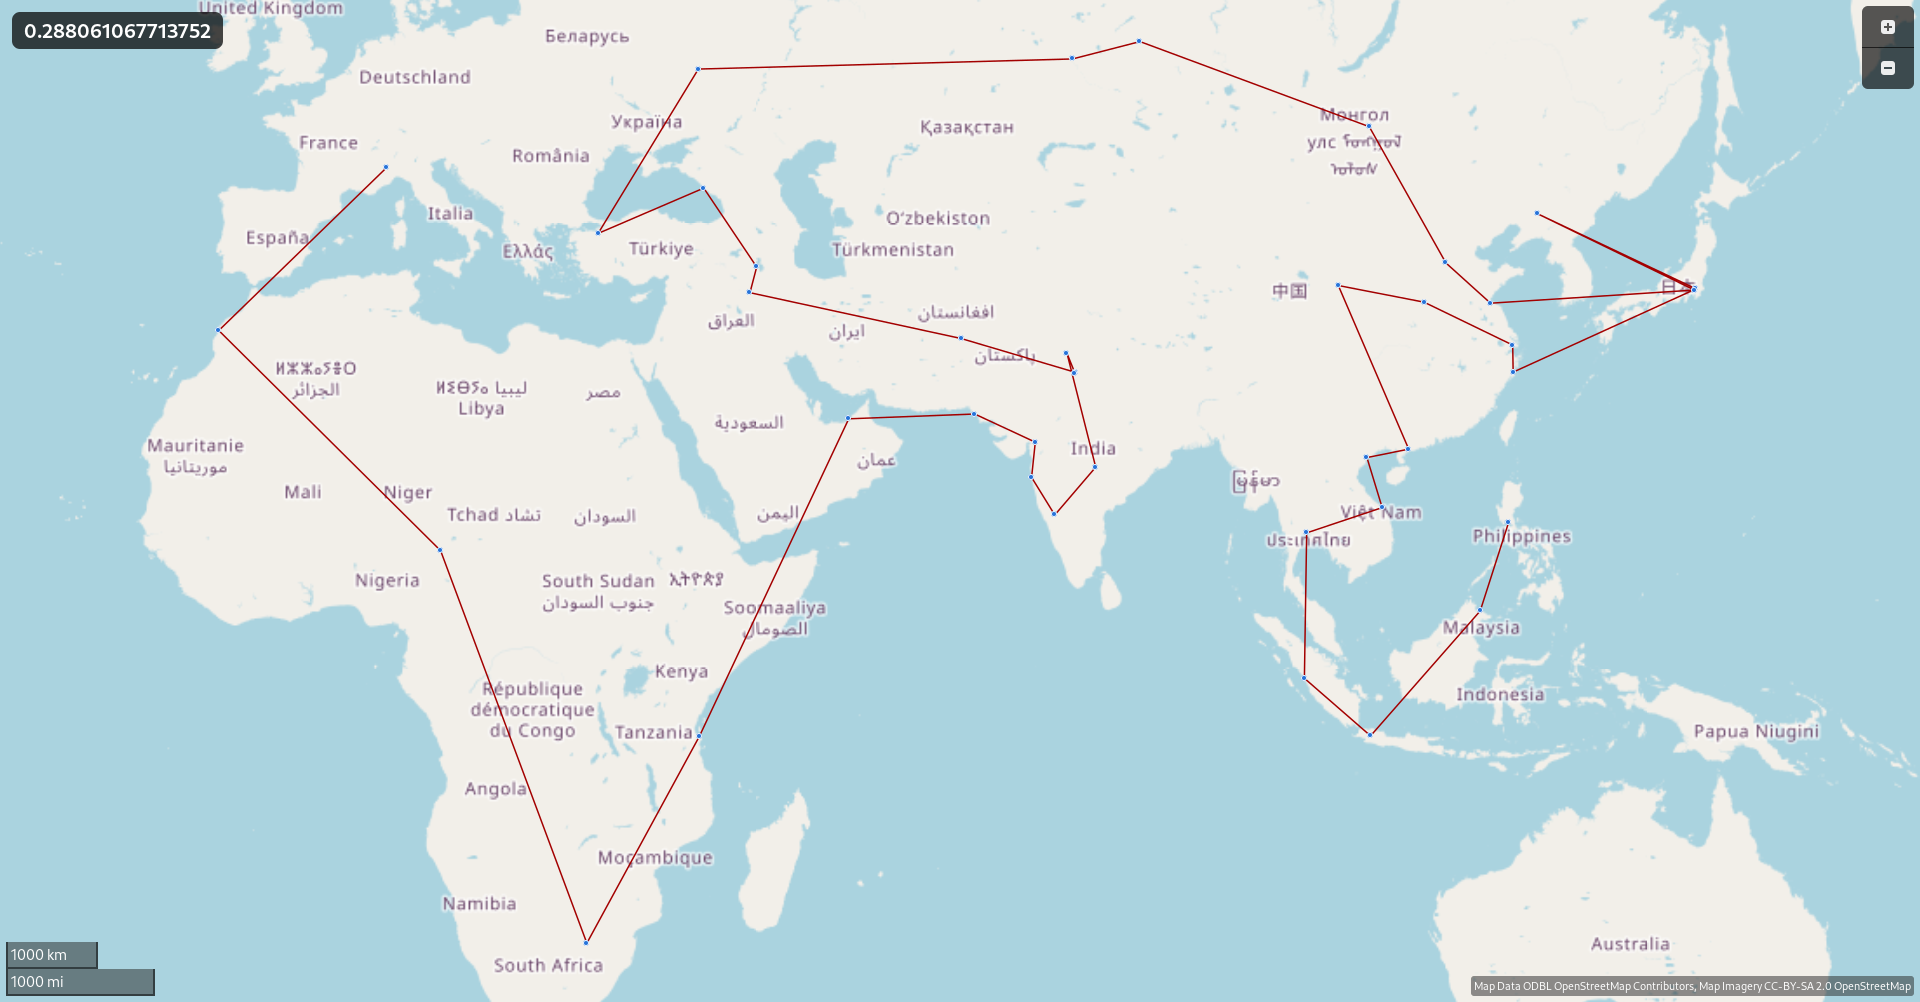
\includegraphics[width=.81\linewidth]{Imágenes/mapa-40.png}
    \caption{Mejor trayectoria para \texttt{input-40}.}
    \label{fig:mapa-40}
\end{figure}

\section{Conclusiones}

La heurística de Aceptación por Umbrales resultó eficaz para encontrar
soluciones factibles a las dos instancias del TSP, alcanzando costos
normalizados de $0.2659$ y $0.1400$. El diseño de la función de costo, que
penaliza las aristas inexistentes en lugar de prohibirlas, permitió que la
búsqueda convergiera de forma natural hacia soluciones factibles sin necesidad
de restricciones explícitas.

La experimentación considero fue lo más importante para poder obtener valores variados y en algún punto llegar a uno lo suficientemente bueno, observamos que la calidad de las soluciones depende fuertemente
de los parámetros, en particular del factor de enfriamiento: valores cercanos a
$1$ producen mejores soluciones a costa de un mayor tiempo de cómputo. 


% Referencias
\clearpage
\nocite{*}
\bibliographystyle{apalike}
\bibliography{Libros.bib}

\centering\vspace*{\fill} 
\end{document}

 %Fin del documento.